\graphicspath{{./figures}}

\section{PocketQube Unit Antenna}
\subsection{Simulation Design}
It was decided to use a simple half-wavelength dipole for the PQ unit, due to its omni-directional radiation pattern and its extremely easy design and construction. The wavelength of interest is for the custom protocol i.e. $f = \SI{433}{MHz}$ or 693 mm. A simple 1.5 mm metal wire will be used due to its availability, with a small gap between the two sides of the dipole, and fed by a coaxial cable.

The design parameters for the dipole are $L_\lambda$ (the total dipole length relative to lambda), $F_{\textnormal{gap}}$ (the gap distance of the feed), and $F_{length}$, the length of the feed. A fixed gap distance of $F_{\textnormal{gap}} = \SI{5}{mm}$ is decided on, as it is assumed to not be critical if sufficiently small.

\begin{figure}[!htb]
  \begin{minipage}{.49\textwidth}
    \centering
    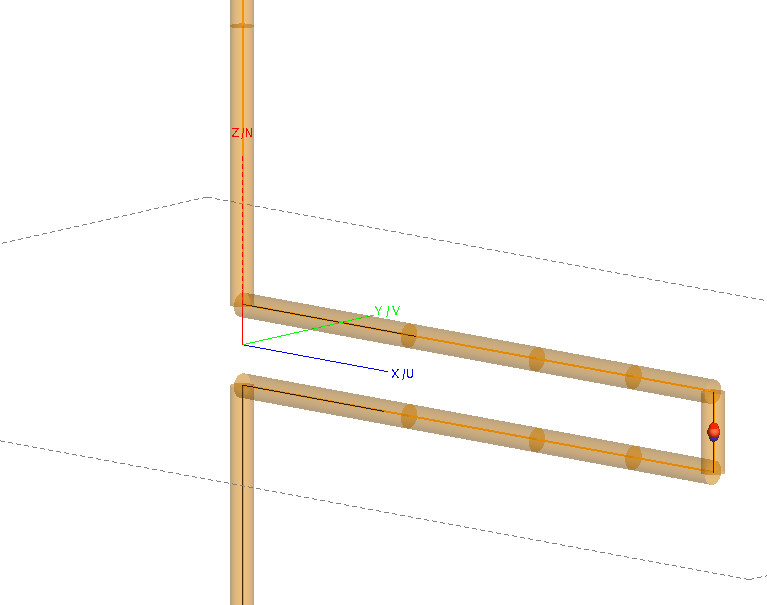
\includegraphics[width=0.65\linewidth]{dipole1_modelMesh}
    \caption{Dipole Model}
    \label{fig:dipole1_modelMesh}
  \end{minipage}
  \begin{minipage}{.49\textwidth}
    \centering
    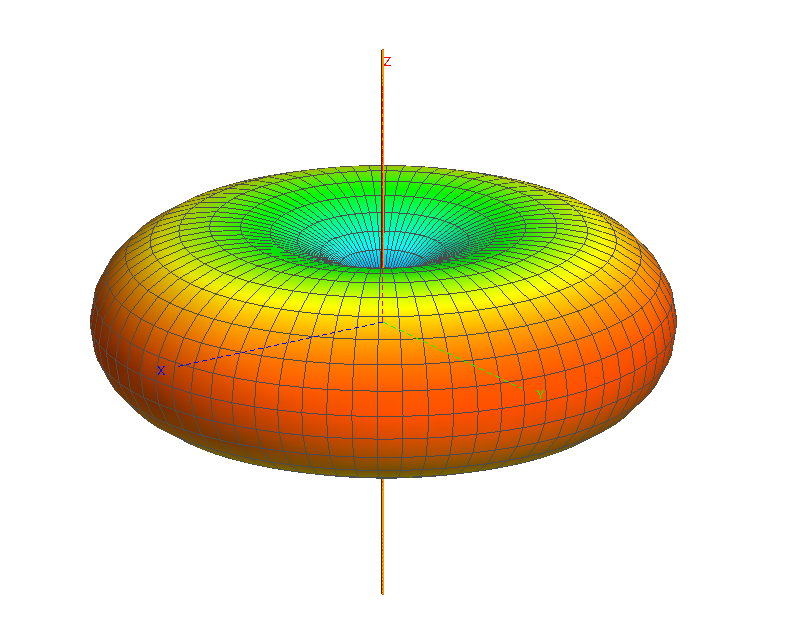
\includegraphics[width=0.65\linewidth]{dipole1_pattern_433MHz}
    \caption{$0.45 \lambda$ Dipole Radiation Pattern}
    \label{fig:dipole1_pattern_433MHz}
  \end{minipage}
\end{figure}

The FEKO model in Figure \ref{fig:dipole1_modelMesh} was used. The optimizer was used to calculate the optimal dipole length and feed length that would minimize the return loss for $f = \SI{433}{MHz}$ at a feed impedance of $\SI{50}{\ohm}$. The resultant parameters are found to be $L_\lambda = 0.45$ ($L = \SI{312}{mm}$) and $F_{\textnormal{length}} = \SI{39.0}{mm}$. The resultant radiation pattern of the dipole is shown in Figure \ref{fig:dipole1_pattern_433MHz}, as well as the optimised return loss as a function of frequency in Figure \ref{fig:dipole1_returnLoss}.

\begin{figure}[!htb]
  \centering
  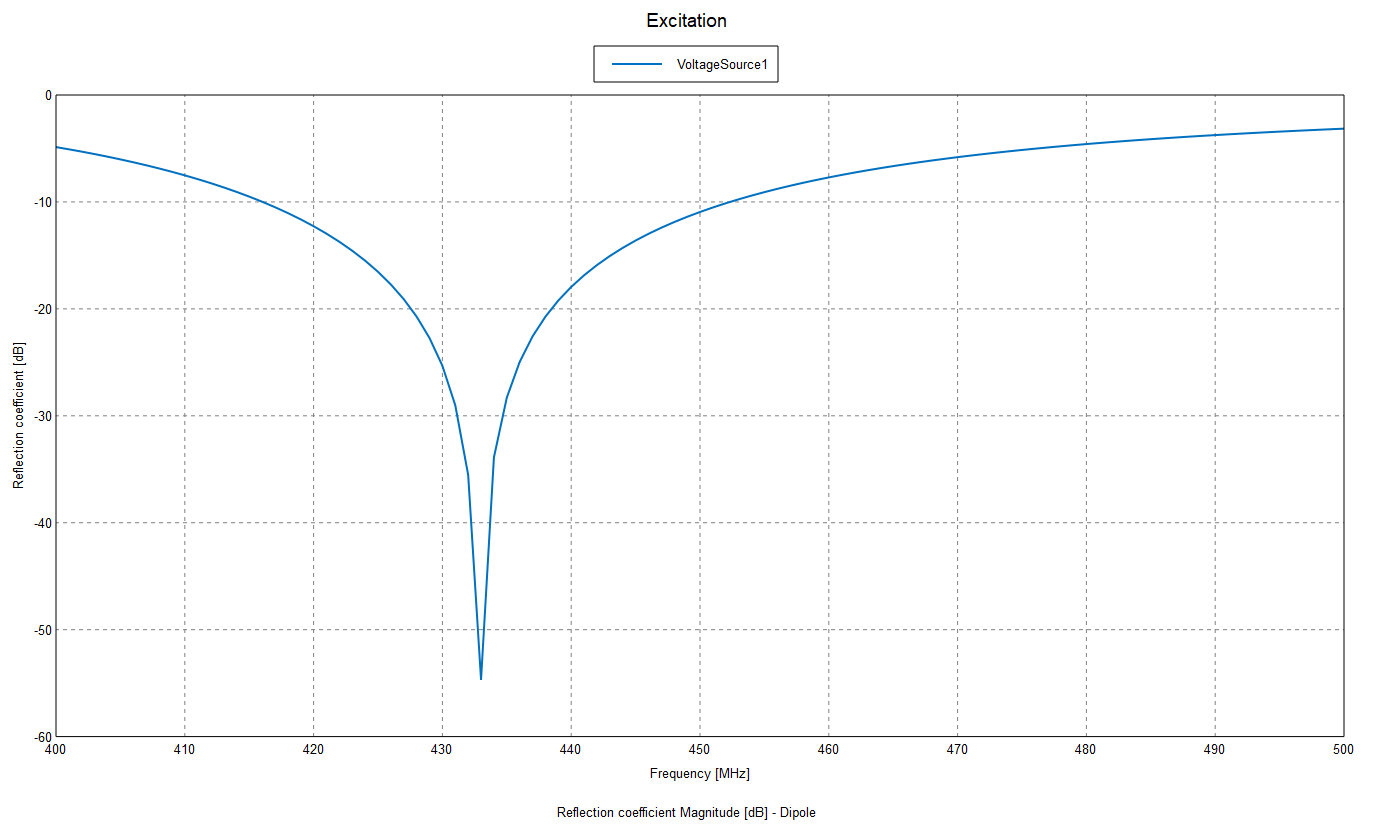
\includegraphics[width=0.65\textwidth]{dipole1_returnLoss}
  \caption{$0.45 \lambda$ Dipole Return Loss vs Frequency}
  \label{fig:dipole1_returnLoss}
\end{figure}